%% Copernicus Publications Manuscript Preparation Template for LaTeX Submissions
%% ---------------------------------
%% This template should be used for copernicus.cls
%% The class file and some style files are bundled in the Copernicus Latex Package, which can be downloaded from the different journal webpages.
%% For further assistance please contact Copernicus Publications at: production@copernicus.org
%% https://publications.copernicus.org/for_authors/manuscript_preparation.html

%% copernicus_rticles_template (flag for rticles template detection - do not remove!)

%% Please use the following documentclass and journal abbreviations for discussion papers and final revised papers.

%% 2-column papers and discussion papers
\documentclass[gc, manuscript]{copernicus}



%% Journal abbreviations (please use the same for preprints and final revised papers)

% Advances in Geosciences (adgeo)
% Advances in Radio Science (ars)
% Advances in Science and Research (asr)
% Advances in Statistical Climatology, Meteorology and Oceanography (ascmo)
% Annales Geophysicae (angeo)
% Archives Animal Breeding (aab)
% Atmospheric Chemistry and Physics (acp)
% Atmospheric Measurement Techniques (amt)
% Biogeosciences (bg)
% Climate of the Past (cp)
% DEUQUA Special Publications (deuquasp)
% Drinking Water Engineering and Science (dwes)
% Earth Surface Dynamics (esurf)
% Earth System Dynamics (esd)
% Earth System Science Data (essd)
% E&G Quaternary Science Journal (egqsj)
% EGUsphere (egusphere) | This is only for EGUsphere preprints submitted without relation to an EGU journal.
% European Journal of Mineralogy (ejm)
% Fossil Record (fr)
% Geochronology (gchron)
% Geographica Helvetica (gh)
% Geoscience Communication (gc)
% Geoscientific Instrumentation, Methods and Data Systems (gi)
% Geoscientific Model Development (gmd)
% History of Geo- and Space Sciences (hgss)
% Hydrology and Earth System Sciences (hess)
% Journal of Bone and Joint Infection (jbji)
% Journal of Micropalaeontology (jm)
% Journal of Sensors and Sensor Systems (jsss)
% Magnetic Resonance (mr)
% Mechanical Sciences (ms)
% Natural Hazards and Earth System Sciences (nhess)
% Nonlinear Processes in Geophysics (npg)
% Ocean Science (os)
% Polarforschung - Journal of the German Society for Polar Research (polf)
% Primate Biology (pb)
% Proceedings of the International Association of Hydrological Sciences (piahs)
% Safety of Nuclear Waste Disposal (sand)
% Scientific Drilling (sd)
% SOIL (soil)
% Solid Earth (se)
% The Cryosphere (tc)
% Weather and Climate Dynamics (wcd)
% Web Ecology (we)
% Wind Energy Science (wes)

% Pandoc citation processing

% The "Technical instructions for LaTex" by Copernicus require _not_ to insert any additional packages.
% 
% tightlist command for lists without linebreak
\providecommand{\tightlist}{%
  \setlength{\itemsep}{0pt}\setlength{\parskip}{0pt}}


%
\begin{document}


\title{Needs and obstacles relating to Open Science at ITC - Results
from an online questionnaire}


\Author[1, *]{Markus}{Konkol}


\affil[1]{ITC, University of Twente, Enschede, Netherlands}

\runningtitle{Results of the Online Questionnaire}

\runningauthor{Konkol}


\correspondence{Markus\ Konkol\ (m.konkol@utwente.nl)}



\received{}
\pubdiscuss{} %% only important for two-stage journals
\revised{}
\accepted{}
\published{}

%% These dates will be inserted by Copernicus Publications during the typesetting process.


\firstpage{1}

\maketitle


\begin{abstract}
Open Science (OS) is becoming increasingly important, but its success
strongly depends on how well the barriers (e.g., knowledge gaps) are
tackled. We conducted an online questionnaire to investigate which
obstacles prevent ITC's researchers from adhering to OS principles and
at which stage of the research cycle they need support. Based on the
insights, we provide a list of recommendations to establish a
transparent, verifiable, and reusable way of doing research.
\end{abstract}


\copyrightstatement{The software is licensed under MIT, the report under
CC-BY, and the dataset under CC0.}


\section{Introduction}

The Faculty of Geo-Information Science and Earth Observation (ITC) at
the University of Twente in the Netherlands endorsed
\href{https://doi.org/10.5281/zenodo.5113578}{\color{blue}{ITC’s Strategic Plan for Open Science 2021-2025 - Towards an Open Future}}
\citep{konkol2021itc} as a starting point to establish faculty-wide Open
Science (OS) practices. Moreover, OS has become part of
\href{https://www.itc.nl/about-itc/itc-mission-and-vision-2020-2030.pdf}{\color{blue}{ITC’s mission and vision}}.
OS is an umbrella term covering several practices to make research more
transparent, verifiable, and re-usable. These practices comprise
\textit{Open Scientific Knowledge} (incl.~openly available scientific
articles, data, software, hardware, and educational materials),
\textit{OS Infrastructures} (incl.~repositories and computational
infrastructures), \textit{Open Engagement of Societal Actors}
(incl.~Citizen and Participatory Science), and
\textit{Open Dialogue with other Knowledge Systems} (see
\href{https://en.unesco.org/science-sustainable-future/open-science/recommendation}{\color{blue}{UNESCO's Recommendation on OS}}
\citep{unesco} for a full definition). The OS plan aims to assist ITC in
realising an open research environment through five initiatives:

\begin{enumerate}
\def\labelenumi{\arabic{enumi}.}
\tightlist
\item
  \textit{Open Science at ITC} is about developing guidelines and
  capacity building.
\item
  \textit{The ITC Knowledge Hub} is about developing tools and
  installing services to facilitate OS.
\item
  \textit{Open Educational Resources} is about exploring options to open
  up teaching materials.
\item
  \textit{The Open Science Community Twente} is about providing a space
  to promote, learn, and discuss OS practices.
\item
  \textit{Research and Funding} is about hiring staff to share
  responsibility and carry out user studies.
\end{enumerate}

This document is part of the first initiative
\textit{Open Science at ITC}, which aims to train ITC researchers in OS
practices and address the obstacles they encounter when doing OS. To
achieve this aim, we approached the researchers of the six departments
at ITC\footnote{ITC's departments: Earth Observation Science
  (\href{https://www.itc.nl/about-itc/organization/scientific-departments/earth-observation-science/profile/}{EOS}),
  Applied Earth Science
  (\href{https://www.itc.nl/about-itc/organization/scientific-departments/earth-systems-analysis/}{AES}),
  Geo-Information Processing
  (\href{https://www.itc.nl/about-itc/organization/scientific-departments/geo-information-processing/}{GIP}),
  Natural Resources
  (\href{https://www.itc.nl/about-itc/organization/scientific-departments/natural-resources/profile/}{NRS}),
  The Urban and Regional Planning and Geo-information Management
  department
  (\href{https://www.itc.nl/about-itc/organization/scientific-departments/urban-regional-planning-geo-information-management/profile/}{PGM}),
  Water Resources
  (\href{https://www.itc.nl/about-itc/organization/scientific-departments/water-resources/profile/}{WRS})}
with an online survey to answer the following questions:

\begin{enumerate}
\def\labelenumi{\arabic{enumi}.}
\item
  In which OS practices are researchers at ITC interested?
\item
  Which obstacles prevent ITC researchers from doing OS?
\item
  At which stage of the research process do ITC researchers need support
  relating to OS?
\end{enumerate}

The insights will be used to plan, prioritise, and carry out concrete
activities to tackle barriers and fill knowledge gaps around OS. In the
following chapters, we first report on the methodology and the results.
Afterwards, we discuss the findings and conclude by suggesting concrete
activities to establish OS at ITC.

\section{Methodology}

\subsection{Questionnaire}

First, the questionnaire provided a brief introduction of what OS means,
who is addressed by the survey, and what its goals are. Then, the
questionnaire collected background information from the participants,
i.e., department, current research position (postdoc,
assistant/associate/full professor, Ph.D.~candidate employed at ITC or
with a scholarship), and how many years they have spent in research so
far. Afterwards, the questionnaire asked for the participants' degree of
agreement with the statement
`\textit{I would like to learn more about...}' followed by a set of OS
practices based on
\href{https://unesdoc.unesco.org/ark:/48223/pf0000374409}{UNESCO's
Recommendation on OS} (e.g., Open Data, Open Code and Methods
etc.)\footnote{Note: The listed OS practices are aligned with the first
  draft of UNESCO's Recommendation on OS that was released in 2020. In
  2021, an
  \href{https://en.unesco.org/science-sustainable-future/open-science/recommendation}{updated
  version} has been published which includes slightly different terms.}
on a five-point Likert scale ranging from strongly disagree to strongly
agree. Subsequently, participants gained a list of common obstacles
relating to OS (e.g., \textit{It takes too much time}) and were asked to
tick those that hinder them from doing OS. If the participants ticked an
obstacle, they optionally could provide a more detailed explanation as a
free text. Afterwards, we asked at which stage of the research process
they need support in terms of OS (e.g., while
\textit{processing and analysing data}). Finally, participants were
given the opportunity to provide general comments. The questionnaire was
created using
\href{https://www.limesurvey.org/de/}{\color{blue}{LimeSurvey}}, an open
source online survey tool. The final questionnaire is available in the
supplements.

The results were analysed with the help of descriptive statistics. Free
text answers were analysed using open coding. We first extracted key
statements from the comments, labelled them using codes, and finally
categorised these codes to higher-level themes. The survey was online
from 30th April, 2021 until 11th August, 2021.

\subsection{Participants}

The questionnaire was promoted via faculty-internal announcements
(similar to a newsletter) and the
\href{https://www.itc.nl/research/open-science/about/user-committee/}{\color{blue}{OS@ITC User Committee}}
who forwarded the questionnaire to their departments. Since the response
rate was low during the first five weeks (\textasciitilde30 responses),
we contacted researchers personally via an online messenger to remind
them about the survey.

To ensure anonymity, personal information on position and years in
research are reported in an aggregated way and were removed from the
dataset. In addition, free text answers were checked for details that
might lead to the identification of the participant and replaced by
higher-level descriptors, e.g., ``\textit{[company]}'' instead of the
name of the company.

We removed three participants from the dataset, two of them because they
were not affiliated as researchers with one of the six departments and
one because the participant was a lecturer. In total, 90 participants
completed the survey, including 14 from EOS, 15 from AES, 14 from GIP,
16 from NRS, 17 from PGM, and 14 from WRS. The cohort was composed of 25
assistant professors, 20 Ph.D.~candidates employed at ITC, 16
Ph.D.~candidates with a scholarship, 10 associate professors, 11
postdocs, and 8 full professors. On average, the participants have spent
6,5 years in research.

\section{Results}

This section summarises the results of the survey. The materials (data
and source code) are available in the supplements.

\subsection{In which OS practices are researchers at ITC interested?}

From all OS practices (see Figure 1), researchers at ITC are mostly
interested in Open Reproducible Research (80\% agreed or strongly
agreed), Open Data (78\%), Open Educational Resources (78\%), Open Code
and Methods (77\%), and Open Infrastructure (77\%). Also, Open Access
and Preprints (72\%), Open-Source Software and Hardware (72\%), and
Openness to Diversity and Inclusivity (72\%) reached high ratings.
Around two-thirds would like to learn about Open Licenses (69\%), Open
Evaluation (e.g.,
\href{https://sfdora.org/}{\color{blue}{San Francisco Declaration on Research Assessment}})
(68\%), and Citizen and Participatory Science (63\%). Around half of the
participants are interested in Open Peer Review (57\%) and
Pre-registration and Registered Reports (47\%).

Generally, there is little disinterest in OS practices. Around one in
ten are not interested in learning about Open Peer Review (11\%), Open
Access and Preprints (10\%), Preregistration and Registered Reports
(10\%), Citizen and Participatory Science (9\%), Open Evaluation (8\%),
and Openness to Diversity and Inclusivity (8\%). The remaining values
range from 3\% to 6\%.

The number of those who neither agree nor disagree differs substantially
among the OS practices. Pre-registration and Registered Reports have the
highest score (43\%) followed by Open Peer Review (32\%), Citizen and
Participatory Science (28\%), and Open Licenses (26\%). These high
values might indicate knowledge gaps making it difficult for the
participants to say whether the corresponding practice is important for
them or not. For the remaining OS practices, around one in five neither
agrees nor disagrees.

\begin{figure}
\centering
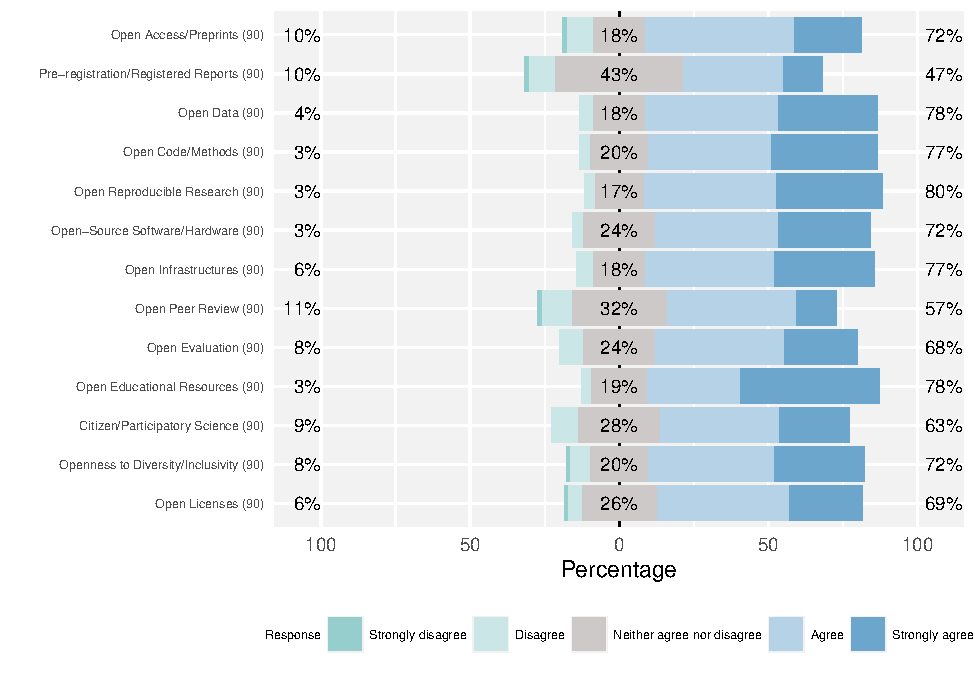
\includegraphics{questionnaire_files/figure-latex/unnamed-chunk-5-1.pdf}
\caption{Degree of agreement to the statement: `I would like to learn
more about\ldots{}' followed by the listed OS practices (90
respondents).}
\end{figure}

\subsection{Which obstacles prevent ITC researchers from doing OS?}

Table 1 shows how many participants (overall and per
department\footnote{Note: The differentiation by department is not meant
  for blaming, but to prioritise activities and provide custom-tailored
  support and advise.}) face the corresponding obstacle when doing OS,
ordered by the overall occurrence. In total, the participants ticked the
16 obstacles 235 times (2,6 obstacles per participant). In the
following, we complement the numbers from the table with the written
statements made by the participants.

\begin{table}
\caption{Number of participants (overall and per department) facing the corresponding obstacle when doing OS, ordered by occurrence.}
\begin{tabular}{p{9cm} | p{0.6cm} | p{0.6cm} | p{0.6cm} | p{0.6cm} | p{0.6cm} | p{0.6cm} | p{0.6cm}} 
\textbf{Obstacles} & \textbf{All} & \textbf{EOS} & \textbf{AES} & \textbf{GIP} & \textbf{NRS} & \textbf{PGM} & \textbf{WRS} \\
\hline
1) It takes too much time and work & 31 & 6 & 5 & 5 & 5 & 4 & 6 \\
\hline
2) I work with sensitive data & 26 & 3 & 6 & 5 & 3 & 8 & 1 \\
\hline
3) I do not know how to license data and code & 24 & 1 & 3 & 7 & 4 & 7 & 2 \\
\hline
4) I use commercial software & 23 & 2 & 6 & 3 & 4 & 5 & 3 \\
\hline
5) The pressure to publish & 22 & 2 & 1 & 4 & 7 & 2 & 6 \\
\hline
6) Lack of funding & 14 & 3 & 0 & 3 & 4 & 1 & 3 \\
\hline
7) I do not know how & 14 & 0 & 2 & 4 & 4 & 2 & 2 \\
\hline
8) The company/institution I am working with does not allow sharing & 13 & 2 & 3 & 3 & 3 & 0 & 2 \\
\hline
9) My materials may be misinterpreted & 11 & 2 & 1 & 2 & 1 & 4 & 1 \\
\hline
10) It was not yet relevant & 10 & 0 & 3 & 1 & 1 & 4 & 1 \\
\hline
11) I do not want to lose my competitive advantage & 10 & 1 & 1 & 1 & 5 & 0 & 2 \\
\hline
12) I do not think that others will need the materials & 9 & 1 & 0 & 1 & 4 & 2 & 1 \\
\hline
13) Because of copyright concerns & 8 & 1 & 2 & 3 & 0 & 1 & 1 \\
\hline
14) I do not know where to publish my materials & 8 & 1 & 2 & 1 & 2 & 1 & 1 \\
\hline
15) My materials may be misused & 7 & 0 & 1 & 1 & 1 & 3 & 1 \\
\hline
16) The tools are missing & 5 & 0 & 4 & 1 & 0 & 0 & 0 \\
\hline
Sum & 235 & 25 & 40 & 45 & 48 & 44 & 33 \\
\hline
\end{tabular}
\label{table:1}
\end{table}

\textit{\textbf{Effort}}: For most participants, OS takes too much time
and work (31 ticked this obstacle). This issue seems to emerge
consistently across departments. Most of the participants' comments
referred to reproducible research (13 participants made a statement that
falls under this category), e.g., rewriting source code to facilitate
understanding and reuse. Several statements fall under the category FAIR
and open data (10), such as documentation and converting closed to open
data formats. Another set of statements referred to rewards and
recognition (6). One participant stated:

\begin{quote}
\textit{"Once a paper is finally published, there are so many other tasks that prevent from taking time and storing data."}
\end{quote}

Another participant addressed the research cycle:

\begin{quote}
\textit{"It needs to be taken more explicitly into account at the beginning. Now it is often an overlooked after-burner."}
\end{quote}

Extra effort is also an issue when it comes to finding and learning new
open source software to replace familiar but commercial tools (2). One
participant referred to open educational resources, saying that it takes
time to get the permission from the directorate to publish open
courseware.

\textit{\textbf{Sensitive data}}: The work with sensitive data is
another often-ticked barrier (26), particularly in the PGM (8), AES (6),
and GIP (5) department. The participants named three reasons:
Predominantly, privacy and ethics regulations prevent researchers from
sharing data (18). Furthermore, the data provider sometimes restricts
data sharing (4), but also collaborators (e.g., partners, companies) do
so (3). One participant stated:

\begin{quote}
\textit{"Sometimes I work with secondary data from partners who do not want their data to be made available."}
\end{quote}

\textit{\textbf{Licensing}}: A further issue is not knowing how to
license data and code (24), which is predominantly an issue at GIP (7),
PGM (7), and NRS (4). The comments show a lack of understanding and
doubts whether licenses are relevant:

\begin{quote}
\textit{"What I know I have learned from practice, but it is not sufficient, and sometimes also confusing."}
\end{quote}

\begin{quote}
\textit{"I do not think this is necessary in my case. I share my code to people who need it."}
\end{quote}

One participant struggles with licenses when it comes to determining
whether someone else's work can be reused.

\textit{\textbf{Commercial software}}: Many respondents make use of
commercial software (23), particularly at AES (6), PGM (5), and NRS (4).
Most participants use a commercial programming software, i.e., MATLAB
(5) and IDL (5). Furthermore, ESRI software (9) for GIS purposes and
ERDAS (6) for remote sensing analyses are popular tools. Envi (4) is
used as an image processing and analysis tool, eCognition (3) for image
analysis and Pix4D (3) for photogrammetry. Further tools in use are
AtlasTI (1) for the analysis of qualitative data, Maptionnaire (1) for
creating map-based surveys, Office Timeline Pro (1) for project
management, SPSS (1) for statistics, Google Earth Engine (1) for
geospatial processing services, HoloLens 2 (1) for augmemnted reality
applications, and Visual Studio (1) as an interactive programming
environment.

\textit{\textbf{Pressure to publish}}: The pressure to publish is a
crucial issue (22), mostly at NRS (7) and WRS (6). Most comments
referred to missing rewards and recognition (7), resulting in missing
incentives to invest effort in OS practices. One participant stated:

\begin{quote}
\textit{"Most time is spent to get an accepted publication out, rather than a published accompanying dataset or code."}
\end{quote}

The journal impact factor plays a role as well:

\begin{quote}
\textit{"Unfortunately, most of the journals with higher impact factor (required for project acquisition and other achievements) are not open access yet."}
\end{quote}

The statements also revealed an interesting range of mindsets. While one
participant
\textit{"open[s] repos only after the acceptance of the paper"}, another
stated:

\begin{quote}
\textit{"It is a very bad idea to ask the ongoing PhD students to share and publish their research data."}
\end{quote}

Unfortunately, the person making the latter statement missed to provide
an elaborated answer and concrete arguments.

\textit{\textbf{Lack of funding}}: Missing funding was ticked 14 times.
Most of the comments refer to Open Access (4), which requires funding.
However, from the comments it was not always clear whether the
participants referred to costs relating to article processing charges or
releasing data and code:

\begin{quote}
\textit{"When publishing parallel work, the lack of funding prevents me from publishing open access."}
\end{quote}

Two participants see OS as an extra activity that is not part of the
actual research and thus requires extra funding:

\begin{quote}
\textit{"OS may require funding support for extra activities that are not normally included during a PhD."}
\end{quote}

\textit{\textbf{Lack of knowledge}}: Missing knowledge was ticked 14
times, mostly people from NRS (4) and GIP (4). The comments did not
reveal concrete knowledge gaps but rather a general lack of awareness of
OS practices (6). For instance, one participant has not much experience
with sharing data, and another one is not familiar with sharing
reproducible code.

\textit{\textbf{Restrictions by the company/institution}}: 13
participants indicated that cooperating with companies or institutions
that do not allow data sharing is an obstacle. This issue occurs
consistently across departments, except PGM. From those who commented,
five participants worked with a company that restricted sharing, two
with a research unit, and one with an unspecified organisation. One
participant stated:

\begin{quote}
\textit{"I have industry partners in my research who want to commercialize the results or to keep the data."}
\end{quote}

Apparently, there is a trade-off between adhering to OS principles and
learning commercial software needed in industry as one participant
stated:

\begin{quote}
\textit{"This was the case when I worked with the industry, there I acquired most of my skills which are based on licences."}
\end{quote}

\textit{\textbf{Misinterpretation of materials}}: 11 out of 90 fear
their materials might be misinterpreted, most coming from PGM (4). An
essential issue relates to the context of qualitative data (e.g., space,
time, personal/environmental circumstances), which was mentioned two
times. One participant stated:

\begin{quote}
\textit{"This is a major concern for the qualitative data that I am collecting. People who are not familiar with the context will not be able to interpret it well."}
\end{quote}

\textit{\textbf{Not yet relevant}}: It was not yet relevant say ten
participants (PGM (4), AES (3)). For two participants, it was not yet
relevant since they were not aware of OS practices:

\begin{quote}
\textit{"The issue of OS has been very raised recently - at least to my knowledge - I don't feel familiar with many aspects."}
\end{quote}

According to one participant, the software is too specific and was
developed for a unique case. Finally, for one participant it was not yet
relevant due to missing rewards and recognition.

\textit{\textbf{Competitive advantage}}: The fear of losing the
competitive advantage is an obstacle for ten participants. For one
participant, this is especially relevant if big data is involved.
Another participant uses embargo periods to mitigate this threat. One
participant stated:

\begin{quote}
\textit{"There is usually a little bit of this (old-fashioned) sentiment."}
\end{quote}

\textit{\textbf{Remaining obstacles}}: Nine participants think others
will not need the materials, since the code is not understandable or the
data too specific:

\begin{quote}
\textit{"This is exaggerated but I don't even understand my own code, hard to imagine it can be of use for others."}
\end{quote}

\begin{quote}
\textit{"I am unsure how far the data I collect is relevant for other studies. It is quite time and place specific."}
\end{quote}

Eight respondents have concerns regarding copyright. This issue applies
to teaching but also in a more general setting:

\begin{quote}
\textit{"Some of my teaching materials may contain copyrighted materials/contributions from previous lecturers and may not be readily shared."}
\end{quote}

\begin{quote}
\textit{"Maybe I use others' open code and they have specific requirements for re-share the code."}
\end{quote}

Eight participants do not know where to publish the materials, including
a limited understanding of data repositories like DANS. Seven fear their
materials might be misused. Two participants commented that open data
can result in negative implications for their participants:

\begin{quote}
\textit{"Some of the data we collected despite not being personal it can be used and have negative consequences for the participants who trusted us."}
\end{quote}

Finally, five participants criticize the lack of tools, which is mainly
an issue for researchers at AES (4):

\begin{quote}
\textit{"Not everything is available open or can be developed that easily, as generic functions are usually available as OSS [=open source software] but very task specific ones not."}
\end{quote}

\subsection{At which stage of the research process do ITC researchers
need support relating to OS?}

Table 2 shows how many participants (overall and per department) need OS
support at different stages of the research cycle. Overall, the listed
research stages were ticked 293 times (3,3 ticked research stages per
participant). 38 out of 90 participants require OS support while
preparing a data management plan for funding that adheres to OS
principles. Most of them come from PGM (11) followed by AES (7) and WRS
(6). Pre-registering a study or writing a registered report was ticked
by 26. OS support during data collection is needed by 20 participants,
most coming from GIP (5) and PGM (5). The lowest amount of participants
need OS support when (pre-)processing and analysing data (17), including
five from GIP and five from PGM. A large number of participants need OS
support during the storing and long-term preservation of data and
results (45), and when choosing a license for their materials (44). OS
support while publishing preprints is needed by 25 participants and
while publishing articles by 21 participants. 37 participants need OS
support when publishing the materials underlying the results (i.e., data
and code) and 20 participants while re-using others' work.

\begin{table}
\caption{Number of participants (overall and per department) thinking that they need OS support during the corresponding stage of the research process.}
\begin{tabular}{p{9cm} | p{0.6cm} | p{0.6cm} | p{0.6cm} | p{0.6cm} | p{0.6cm} | p{0.6cm} | p{0.6cm}} 
\textbf{Research stage} & \textbf{All} & \textbf{EOS} & \textbf{AES} & \textbf{GIP} & \textbf{NRS} & \textbf{PGM} & \textbf{WRS} \\
  \hline 
  Preparing a data management plan for funding that adheres to OS principles &  38 & 4 & 7 & 5 & 5 & 11 & 6 \\ 
  \hline
  Preregistering a study/Writing a registered report & 26 & 3 & 6 & 5 & 3 & 7 & 2 \\ 
  \hline
  Collecting data & 20 & 2 & 2 & 5 & 2 & 5 & 4 \\ 
  \hline
  (Pre-) Processing and analysing data & 17 & 1 & 2 & 5 & 1 & 5 & 3 \\
  \hline
  Storing and long-term preservation of data and results & 45 & 6 & 8 & 7 & 9 & 7 & 8 \\
  \hline
  Choosing a license for data/software/papers & 44 & 5 & 10 & 8 & 7 & 9 & 5 \\
  \hline
  Publishing preprints & 25 & 5 & 5 & 6 & 3 & 4 & 2 \\
  \hline
  Publishing the materials underlying the results (i.e., data and code) & 37 & 6 & 8 & 6 & 6 & 7 & 4 \\
  \hline
  Publishing articles & 21 & 4 & 1 & 3 & 4 & 5 & 4 \\
  \hline
  Reusing others’ work & 20 & 4 & 2 & 2 & 2 & 5 & 5 \\
  \hline
  Sum & 293 & 40 & 51 & 52 & 42 & 65 & 43 \\
  \hline
\end{tabular}
\label{table:2}
\end{table}

\section{Discussion}

Overall, the results reveal a conflict: On the one hand, researchers at
ITC have a positive stance on OS and are keen to learn more about open
practices. On the other hand, there are a number of obstacles that
prevent researchers from adhering to OS principles. The main reason is
that OS takes too much time and work. One might argue that time is just
another word for priority, and the priority of researchers is to publish
scientific articles, as reflected in another top obstacle (``the
pressure to publish''). The pressure to publish mainly stems from the
current rewards and recognition system. Hiring, promotion, and tenure
decisions are often based quantitative metrics, such as the Journal
Impact Factor or the h-index. These metrics provide `perverse'
incentives that focus solely on scientific articles and do not consider
the number of published open datasets or code repositories
\citep{bouter2020research}. All that counts are the number of published
articles, in which journals these papers were published, and how often
they were cited. For that reason, several researchers indicated that OS
practices were ``not yet relevant''. Per Seglen argued already in 1997
that the impact factor should not be used for evaluating research
\citep{seglen1997impact}. Nature stated in an editorial that it is time
to remodel the journal factor \citep{natureedit2016}. Others used some
martial words and speak about the slavery of the h-index as a means to
measure the unmeasureable \citep{Kreiner_2016}. And even the developer
of the h-index, Jorge Hirsch, stated that the h-index can fail
spectacularly and have severe unintended negative consequences
\citep{conroy2020s}. The rewards and recognition system was also a
recurring element in the comments made by the participants.

Consequently, researchers often do not see OS as part of their daily
work. Instead, several researchers tend to regard OS as
\textit{"something additional"} that is not part of their work but
happening on top of the \textit{"actual research"}. Several free text
statements confirm this impression
(\textit{"extra funding for extra tasks"}). Hence, OS has a lower
priority for some researchers
(\textit{"there are usually so many other tasks"}) although some
recognise that OS should actually be part of the research cycle from the
beginning to avoid an \textit{"overlooked after-burner"}.

Nevertheless, some of the numbers might be explained by a lack of
awareness. Not knowing how to adhere to OS principles seems to be a
practical issue but it also shows that this knowledge gap was not yet a
problem. Apparently, researchers do not necessarily fail and can still
succeed (publish papers, collect funding, become hired) without
following OS principles. However, current developments show that this
form of practising research will not sustain: Reviewers start asking for
access to the materials \citep{stark2018before}; More funders list OS as
a relevant criterion for granting money; and more universities as well
as governments have put OS on their agenda.

Several researchers have the impression to work in a competitive
environment and thus do not want to lose their competitive advantage by
publishing their research materials. Others cooperate with a company
that does not allow sharing. It is questionable whether a university is
the right place for competition. Instead, collaborations are certainly
more desireable and should be pursued. Still, we cannot expect
researchers to negotiate OS practices with their industry partners.
Finding these partners can be challenging and for understandable reasons
researchers (especially early career researchers) are reluctant to
insist in realising OS practices throughout the research project. They
might be worried that they discourage the company or raise a conflict,
which might block alternative career paths. One possibility to mitigate
this issue is to develop university-wide policies that need to be part
of the agreement between researchers and their industry partners. Such
policies can put the university in a stronger position targeting at
least a compromise in which not all but some materials are released
openly. The degree of openness might depend on who is paying how much
for the research project. Companies can make their own rules if they pay
for the research, but in case of a public funder the guideline is
\textit{publicly funded research should become a public good}. It might
also be worth to make companies aware of the benefits of OS, e.g.,
increased visibility, collaboration opportunities, and open source-based
business models.

Another concern of researchers is that the research materials might be
misused and misinterpreted. These arguments alone can be used as
knock-out arguments. It is always possible to say that the materials may
be misused and misinterpreted. It is up for discussion if a deviating
interpretation is a misinterpretation caused by the lack of contextual
information or rather a differing viewpoint by someone who is less
immersed in the data and the context and thus more objective.
Furthermore, not being able to interpret data raises concerns regarding
the verifiability of the outcomes. Still, if these arguments are
justified appropriately, they can be legitimate reasons to hide
materials.

A critical issue in OS is the use of commercial and open-source
software. The number of open-source software is large and covers a broad
range of topics and functionality. However, many researchers tend to use
the tools they are familiar with or that have a more intuitive user
interface. Switching to open source software is in several cases rather
easy, particularly when it comes to programming languages. For example,
MATLAB and SPSS can be replaced by R or python, and ESRI's ArcGIS can be
easily replaced by QGIS. SPSS might have a more efficient user interface
that makes statistics easier but it remains a black box. In other cases,
switching is rather difficult. For instance, besides some tools under
development (e.g., RQDA), there is not yet a fully functioning and
easy-to-use tool for qualitative analyses.

A key goal of ITC is to help students develop capacity. On the one hand,
following OS principles would mean to promote the use of open-source
software, e.g., QGIS. On the other hand, students should develop a broad
range of skills, which might include proprietary software that is
commonly used in industry and a pre-requisite for many jobs (e.g., ESRI
software). While in such cases a fully trained GIS student should be
able to switch between different GIS software easily, this might not
hold true for other software.

Several participants state that others will not need the materials. One
might ask the provoking question whether the research that is based on
materials that others cannot reuse is valuable at all. Fortunately, in
most cases, the researchers probably just underestimate how useful and
relevant their materials are. Sharing them is thus always helpful and
needed to ensure transparent, verifiable, and reusable research results.

\section{Conclusion}

ITC has a positive stance on OS but there are a number of obstacles that
prevent researchers form adhering to OS principles. To mitigate these
barriers, we suggest the following activities.

\textbf{1. Reward participation in OS training courses}

Students, Ph.D.~candidates, and researchers have a full agenda, which is
why many will not attend OS courses that are not rewarded. Hence, OS
training courses should become part of students' curricular,
Ph.D.~candidates' graduate school, and researchers' teaching
qualification. Attending an OS course might even become a requirement
for tenure and promotion. Such rewarded courses provide a concrete
incentive to learn about OS and foster the culture change towards an
open research environment.

\textbf{2. Change the rewards and recognition system}

The success of OS strongly depends on a rewards and recognition system
that incentivises it. This change cannot be achieved by researchers
alone but needs to be an international effort. An important step is
joining
\href{https://ec.europa.eu/info/news/process-towards-agreement-reforming-research-assessment-2022-jan-18_en}{\color{blue}{EU's process towards an agreement on reforming research assessment}}.
Further efforts can be carried out in parallel, such as considering OS
principles in
\href{https://www.nicebread.de/open-science-hiring-practices/}{\color{blue}{hiring decisions}}.

\textbf{3. Develop faculty-wide guidelines and policies}

Faculty-wide (or even university-wide) guidelines and policies are
needed to make sure that OS becomes part of a researchers daily work.
Nowadays, OS is often seen as an extra task, but not following OS
principles is a shortcut and against good scientific practice. Such
guidelines and policies can address the cooperation between researchers
and companies and the need to provide legitimate reasons for hiding
research materials. The overall guideline should be
\textit{as open as possible, as closed as necessary}, requiring
materials to be open by default and closed only where legitimate reasons
apply.

\textbf{4. Consider OS practices early in the research process}

The impression that OS is labour-intensive is also caused by its
consideration at the very end of the research process when deadlines are
close and time is scarse. Hence, tasks such as rewriting source code to
make it better understandable, documentation, and converting closed to
open data formats become an ``overlooked after-burner''. This issue can
be avoided by considering OS principles and best practices from the
beginning. One opportunity is to make OS practices part of data
management plans. Another possibility is to add OS-related aspects to
the ethical approval process, where researchers need to think their
research plan through anyway.\\
Making (future) researchers aware of open practices early in their
career and research process will also flatten the learning curve in the
next projects.

\textbf{5. Provide OS services}

Researchers should have access to support services that reduce the
effort, close knowledge gaps, suggest open practices (e.g., open-source
instead of closed software or open instead of closed data formats),
propose best practices to improve messy code and the quality of
documentation, and help with licensing. Another service might be
\href{https://www.itc.nl/research/open-science/codecheck/}{\color{blue}{CODECHECK}},
``an OS initiative for the independent execution of computations
underlying research articles to improve reproducibility''
\citep{N_st_2021}. Researchers also need consulting when it comes to
copyright. However, this kind of support requires legal experts.

\textbf{6. Require supplemental materials statement in research articles}

Researchers should add a statement to their articles describing where
the underlying materials can be found and, if applicable, which concrete
and legitimate reasons apply for hiding materials. It might also be
possible to use an embargo if justified appropriately.

\textbf{7. Support a community around OS}

OS is a dynamic area and being up to date can be challenging.
Consequently, a space is needed to receive updates, ask questions, and
discuss concerns. An Open Science Community provides a suitable
environment to cover these needs. However, coordinating such a community
is time-consuming and often voluntary work. Thus, the faculty should
provide financial resources for the coordination of the community.

\textbf{8. Create flagship use cases}

Practices like Open Data and Open Reproducible Research should not be
done just for the sake of openness. It is crucial to highlight the
benefit, i.e, transparency, verifiability, and reusability. Since these
benefits are often anecdotal, it is important to create use cases out of
existing and upcoming publications. These use cases should show what is
possible if all materials are there.



\codedataavailability{The data and the code are available under
\href{https://github.com/MarkusKonk/open_science_at_itc_survey.git}{\color{blue}LINK}} %% use this section when having data sets and software code available



%%%%%%%%%%%%%%%%%%%%%%%%%%%%%%%%%%%%%%%%%%
%% optional

%%%%%%%%%%%%%%%%%%%%%%%%%%%%%%%%%%%%%%%%%%

%%%%%%%%%%%%%%%%%%%%%%%%%%%%%%%%%%%%%%%%%%

%%%%%%%%%%%%%%%%%%%%%%%%%%%%%%%%%%%%%%%%%%
\competinginterests{The author works as an Open Science Officer at
ITC.} %% this section is mandatory even if you declare that no competing interests are present

%%%%%%%%%%%%%%%%%%%%%%%%%%%%%%%%%%%%%%%%%%

%%%%%%%%%%%%%%%%%%%%%%%%%%%%%%%%%%%%%%%%%%

%% REFERENCES
%% DN: pre-configured to BibTeX for rticles

%% The reference list is compiled as follows:
%%
%% \begin{thebibliography}{}
%%
%% \bibitem[AUTHOR(YEAR)]{LABEL1}
%% REFERENCE 1
%%
%% \bibitem[AUTHOR(YEAR)]{LABEL2}
%% REFERENCE 2
%%
%% \end{thebibliography}

%% Since the Copernicus LaTeX package includes the BibTeX style file copernicus.bst,
%% authors experienced with BibTeX only have to include the following two lines:
%%
\bibliographystyle{copernicus}
\bibliography{references.bib}
%%
%% URLs and DOIs can be entered in your BibTeX file as:
%%
%% URL = {http://www.xyz.org/~jones/idx_g.htm}
%% DOI = {10.5194/xyz}


%% LITERATURE CITATIONS
%%
%% command                        & example result
%% \citet{jones90}|               & Jones et al. (1990)
%% \citep{jones90}|               & (Jones et al., 1990)
%% \citep{jones90,jones93}|       & (Jones et al., 1990, 1993)
%% \citep[p.~32]{jones90}|        & (Jones et al., 1990, p.~32)
%% \citep[e.g.,][]{jones90}|      & (e.g., Jones et al., 1990)
%% \citep[e.g.,][p.~32]{jones90}| & (e.g., Jones et al., 1990, p.~32)
%% \citeauthor{jones90}|          & Jones et al.
%% \citeyear{jones90}|            & 1990


\end{document}
